% Graphical Abstract for ChEMBL-PDB Linker
% TikZ figure for ChemRxiv submission
\documentclass[11pt]{article}

\usepackage[utf8]{inputenc}
\usepackage[T1]{fontenc}
\usepackage{lmodern}
\usepackage[paperwidth=18cm,paperheight=10cm,margin=0.3cm]{geometry}
\usepackage{tikz}
\usetikzlibrary{shapes.geometric, arrows.meta, positioning, fit, backgrounds, calc}
\usepackage{xcolor}

% Define custom colors
\definecolor{chemblblue}{RGB}{52, 101, 164}
\definecolor{pdbgreen}{RGB}{78, 154, 6}
\definecolor{outputgold}{RGB}{196, 160, 0}
\definecolor{validationred}{RGB}{164, 0, 0}
\definecolor{linkpurple}{RGB}{117, 80, 123}
\definecolor{lightbg}{RGB}{250, 250, 252}

\pagestyle{empty}

\begin{document}
\centering
\vspace*{\fill}

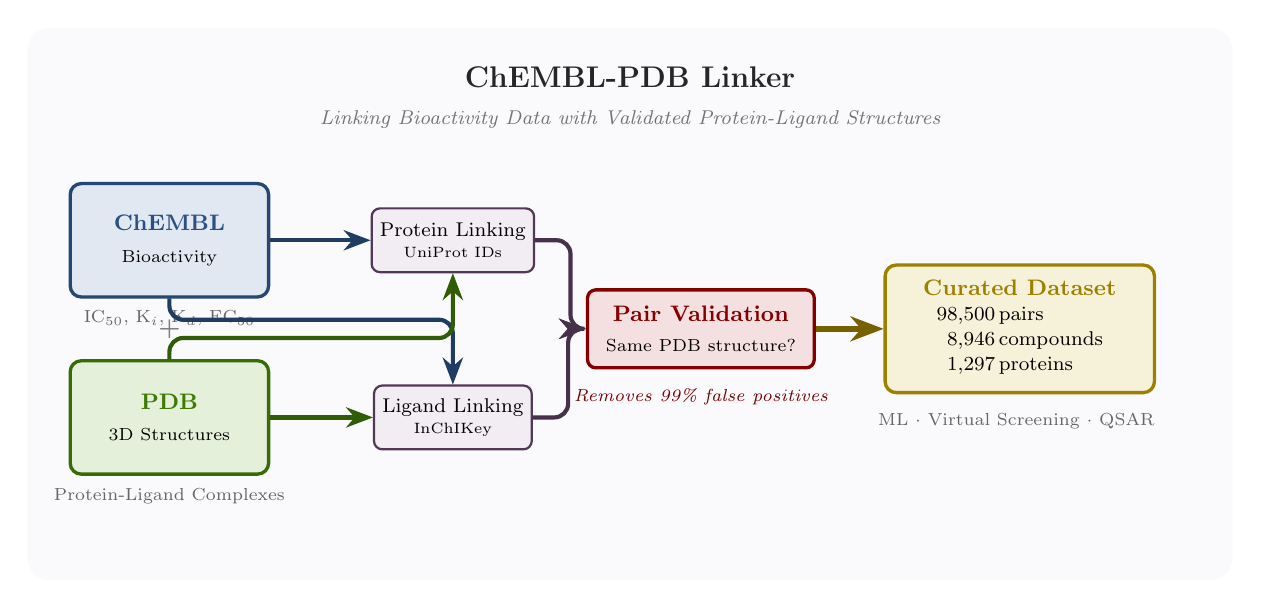
\begin{tikzpicture}[
    scale=0.9,
    transform shape,
    node distance=0.8cm and 1.5cm,
    % Data source boxes
    datasource/.style={
        rectangle,
        draw=#1!70!black,
        fill=#1!15,
        minimum width=2.8cm,
        minimum height=1.6cm,
        align=center,
        rounded corners=4pt,
        font=\small\bfseries,
        line width=1.2pt
    },
    % Process boxes
    process/.style={
        rectangle,
        draw=linkpurple!70!black,
        fill=linkpurple!10,
        minimum width=2.2cm,
        minimum height=0.9cm,
        align=center,
        rounded corners=3pt,
        font=\footnotesize,
        line width=0.8pt
    },
    % Validation box
    validation/.style={
        rectangle,
        draw=validationred!80!black,
        fill=validationred!12,
        minimum width=3.2cm,
        minimum height=1.1cm,
        align=center,
        rounded corners=3pt,
        font=\small\bfseries,
        line width=1.2pt
    },
    % Output box
    output/.style={
        rectangle,
        draw=outputgold!80!black,
        fill=outputgold!15,
        minimum width=3.8cm,
        minimum height=1.8cm,
        align=center,
        rounded corners=4pt,
        font=\small\bfseries,
        line width=1.2pt
    },
    % Arrows
    arrow/.style={
        -{Stealth[scale=1]},
        line width=1.5pt,
        draw=#1!60!black
    },
    % Labels
    datalabel/.style={
        font=\scriptsize,
        align=center,
        text=black!60
    }
]

% Background
\begin{scope}[on background layer]
    \fill[lightbg, rounded corners=8pt] (-6.5,-3.8) rectangle (10.5,4);
\end{scope}

% ===== Title =====
\node[font=\large\bfseries, text=black!85] at (2, 3.3) {
    ChEMBL-PDB Linker
};
\node[font=\footnotesize\itshape, text=black!55] at (2, 2.7) {
    Linking Bioactivity Data with Validated Protein-Ligand Structures
};

% ===== LEFT: Data Sources =====

% ChEMBL Database
\node[datasource=chemblblue] (chembl) at (-4.5, 1) {
    \textcolor{chemblblue!80!black}{ChEMBL}\\[0.15em]
    \fontsize{7}{9}\selectfont\normalfont Bioactivity
};
\node[datalabel, below=0.05cm of chembl] {IC$_{50}$, K$_i$, K$_d$, EC$_{50}$};

% PDB Database
\node[datasource=pdbgreen] (pdb) at (-4.5, -1.5) {
    \textcolor{pdbgreen!80!black}{PDB}\\[0.15em]
    \fontsize{7}{9}\selectfont\normalfont 3D Structures
};
\node[datalabel, below=0.05cm of pdb] {Protein-Ligand Complexes};

% ===== MIDDLE: Linking =====

% Protein linking
\node[process] (protlink) at (-0.5, 1) {
    Protein Linking\\[-0.1em]
    \fontsize{6}{8}\selectfont\normalfont UniProt IDs
};

% Ligand linking
\node[process] (liglink) at (-0.5, -1.5) {
    Ligand Linking\\[-0.1em]
    \fontsize{6}{8}\selectfont\normalfont InChIKey
};

% Validation (center, key innovation)
\node[validation] (validate) at (3, -0.25) {
    \textcolor{validationred!80!black}{Pair Validation}\\[0.1em]
    \fontsize{7}{9}\selectfont\normalfont Same PDB structure?
};

% Filtering label
\node[font=\fontsize{7}{9}\selectfont\itshape, text=validationred!70!black, below=0.15cm of validate] {
    Removes 99\% false positives
};

% ===== RIGHT: Output =====

% Final dataset
\node[output] (dataset) at (7.5, -0.25) {
    \textcolor{outputgold!80!black}{Curated Dataset}\\[0.2em]
    \fontsize{8}{10}\selectfont\normalfont
    \begin{tabular}{r@{\,}l}
        98,500 & pairs\\
        8,946 & compounds\\
        1,297 & proteins
    \end{tabular}
};

% Applications label
\node[datalabel, below=0.15cm of dataset] {
    ML $\cdot$ Virtual Screening $\cdot$ QSAR
};

% ===== ARROWS =====

% ChEMBL to protein linking
\draw[arrow=chemblblue] (chembl.east) -- (protlink.west);

% ChEMBL to ligand linking
\draw[arrow=chemblblue, rounded corners=5pt]
    (chembl.south) -- ++(0,-0.3) -| (liglink.north);

% PDB to protein linking
\draw[arrow=pdbgreen, rounded corners=5pt]
    (pdb.north) -- ++(0,0.3) -| (protlink.south);

% PDB to ligand linking
\draw[arrow=pdbgreen] (pdb.east) -- (liglink.west);

% Protein linking to validation
\draw[arrow=linkpurple, rounded corners=5pt]
    (protlink.east) -- ++(0.5,0) |- (validate.west);

% Ligand linking to validation
\draw[arrow=linkpurple, rounded corners=5pt]
    (liglink.east) -- ++(0.5,0) |- (validate.west);

% Validation to output
\draw[arrow=outputgold, line width=2pt] (validate.east) -- (dataset.west);

% ===== Visual elements =====

% Checkmark on validation
\node[font=\normalsize, text=validationred!80!black] at (1.7, 0.3) {\checkmark};

% Plus sign between sources
\node[font=\bfseries, text=black!50] at (-4.5, -0.25) {+};

\end{tikzpicture}

\vspace*{\fill}
\end{document}
